%%%%%%%%%%%%%%%%%%%%%%%%%%%%%%%%%%%%%%%%%
% Structured General Purpose Assignment
% LaTeX Template
%
% This template has been downloaded from:
% http://www.latextemplates.com
%
% Original author:
% Ted Pavlic (http://www.tedpavlic.com)
%
% Note:
% The \lipsum[#] commands throughout this template generate dummy text
% to fill the template out. These commands should all be removed when 
% writing assignment content.
%
%%%%%%%%%%%%%%%%%%%%%%%%%%%%%%%%%%%%%%%%%

\documentclass{article}

\usepackage{fancyhdr} % Required for custom headers
\usepackage{lastpage} % Required to determine the last page for the footer
\usepackage{extramarks} % Required for headers and footers
\usepackage{graphicx} % Required to insert images
\usepackage[utf8]{inputenc}

% Margins
\topmargin=-0.45in
\evensidemargin=0in
\oddsidemargin=0in
\textwidth=6.5in
\textheight=9.0in
\headsep=0.25in 

\linespread{1.1} % Line spacing



\setlength\parindent{0pt} % Removes all indentation from paragraphs

%----------------------------------------------------------------------------------------
%	DOCUMENT STRUCTURE COMMANDS
%	Skip this unless you know what you're doing
%----------------------------------------------------------------------------------------

% Header and footer for when a page split occurs within a problem environment
\newcommand{\enterProblemHeader}[1]{
\nobreak\extramarks{#1}{#1 continued on next page\ldots}\nobreak
\nobreak\extramarks{#1 (continued)}{#1 continued on next page\ldots}\nobreak
}

% Header and footer for when a page split occurs between problem environments
\newcommand{\exitProblemHeader}[1]{
\nobreak\extramarks{#1 (continued)}{#1 continued on next page\ldots}\nobreak
\nobreak\extramarks{#1}{}\nobreak
}

\setcounter{secnumdepth}{0} % Removes default section numbers
\newcounter{homeworkProblemCounter} % Creates a counter to keep track of the number of problems

%----------------------------------------------------------------------------------------
%	NAME AND CLASS SECTION
%----------------------------------------------------------------------------------------

\newcommand{\lessonNumber}[1]{Lezione\ \##1} % Assignment title
\newcommand{\lessonDate}[4]{#1,\ #2\ #3\ #4} % Due date
\newcommand{\lessonCourse}[1]{#1} % Course/class
\newcommand{\lessonTime}[1]{#1} % Class/lecture time
\newcommand{\lessonTeacher}[1]{#1} % Teacher/lecturer
\newcommand{\lessonAuthor}[1]{#1} % Your name
\begin{document}
\section{Processi Software}
\textbf{Processi software:} attività coordinate, processi di ciclo di vita per far evolvere il sw da uno stato all'altro. Il sw è una macchina a stati che rappresentano il grado di maturazione del prodotto:

\begin{itemize}

	\item \textbf{Concezione}
	\item \textbf{Sviluppo}
	\item \textbf{Utilizzo}
	\item \textbf{Ritiro}

\end{itemize}

Nella fase di ritiro il sw cessa di esistere nel senso che non c'è più alcun tipo di supporto per quel prodotto. Le transizioni sono strettamente e formalmente regolate.	\\

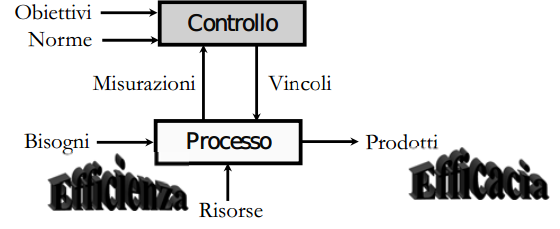
\includegraphics[width=0.75\columnwidth]{img2} % Example image
\\

L'efficienza si vede dove vedo il consumo di risorse. L'efficacia si misura guardando i prodotti e vedendo se sono buoni o cattivi rispetto alla produzione. Un processo è un insieme di attività coordinate e coese (tutti hanno bisogno di tutti).\\
Parole chiave:
\begin{itemize}
	\item\textbf{Iterazione:} iterazione significa operare rivisitazioni o raffinamenti, può essere distruttivo (ripeto l'avanzamento) e rischio di non essere quantificabile.
	\item\textbf{Incremento:} Sono incrementale solo se aggiungo, mi avvicino in maniera monotona all'obbiettivo, non tollera errori o mancanze.
	\item\textbf{Prototipo:}servono per provare e scegliere soluzioni, possono essere o usa e getta o fornire stati di incremento(\textbf{baseline}).
	\item\textbf{Riuso} può essere di due tipi:
	\begin{itemize}
	
		\item occasionale, a basso consto ma a basso impatto.
		\item sistematico, a maggior costo ma a maggior impatto.
	\end{itemize}
	\item \textbf{Manutenzione:} va gestita con il controllo di versione che va ben documentato.
\end{itemize}

Il modello più noto e quello che utilizzeremo e ISO/IEC 12207: questo modello identifica i processi dello sviluppo sw, ne specifica le responsabilità identifica i prodotti di ciascuno.

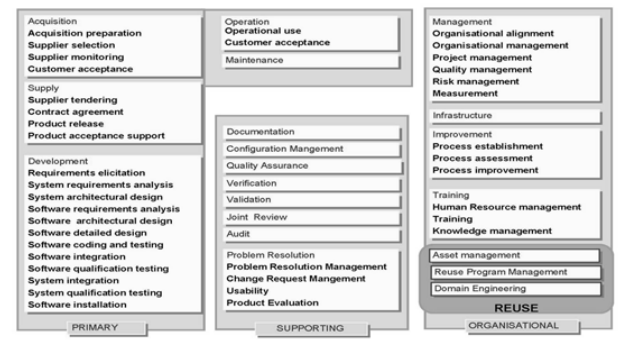
\includegraphics[width=0.75\columnwidth]{img3} % Example image
\\
\textbf{Processi} si dividono in \textbf{Attività} che si dividono in \textbf{Compiti}.

In questo modello ci sono 3 tipi di processi:
\begin{itemize}
	\item \textbf{Processi primari:} che includono processi come Acquisizione(dei propri fornitori), Fornitura(gestione rapporto col cliente), Sviluppo, Manutenzione.
	\item\textbf{Processi di supporto:} che includono processi come Documentazione, Accertamento della qualità, Verifica e Validazione che assieme danno la Qualità, Risoluzione dei problemi
	\item \textbf{Processi organizzativi:} che includono processi come Gestione dei processi, Gestione delle infrastrutture, Formazione del personale, Miglioramento del processo.
\end{itemize}

I processi produttivi devono avere un \textbf{ciclo interno} atto a migliorarli costantemente. Il ciclo interno di miglioramento è indicato con l'acronimo PCDA (o ciclo di Deming). Questo ciclo è fatto di 4 attività che vanno applicate al di "sopra" dei processi esistenti:

\begin{itemize}

	\item \textbf{Plan:} definire attività, scadenze, responsabilità e risorse.
	\item \textbf{Do:} eseguire le attività secondo i piani.
	\item \textbf{Check:} valutare l'esito del processo(in efficacia ed efficienza) rispetto alla pianificazione
	\item \textbf{Act:} applico soluzioni correttive alle carenze rilevate.

\end{itemize}
La scelta del ciclo di vita può essere influenzata da molti aspetti:
\begin{itemize}
	\item politica di sviluppo
	\item natura funzione e sequenza dei processi di revisione per verificare lo stato di avanzamento
	\item necessità di fornire, creare evidenza preliminare di fattibilità(creare prototipi)
	\item evoluzione del sistema e dei suoi requisiti
\end{itemize}

\end{document}
